\documentclass[a4paper,10pt,twocolumn]{article}

\usepackage[utf8]{inputenc}
\usepackage{amsmath}
\usepackage{graphicx}
\usepackage{hyperref}
\usepackage{float}
\usepackage[margin=0.5in]{geometry}
\usepackage{subcaption}

\title{URL Coursework 1: Clustering \\ \Large{Agglomerative clustering via maximum \\ incremental path integral~\cite{PIC}}}
\author{Bruno Sánchez Gómez}
\date{\today}

\begin{document}

\twocolumn[
\maketitle
\begin{abstract}
    This report presents a comprehensive reproduction of the Path Integral Clustering (PIC) algorithm introduced by Zhang et al \cite{PIC}. PIC leverages concepts from statistical physics to effectively cluster data with complex manifold structures by measuring connectivity through path integrals. We implement the algorithm and evaluate it against eleven state-of-the-art clustering methods on both synthetic and real-world imagery datasets (MNIST, USPS, and Caltech-256). Our experiments confirm PIC's exceptional performance, achieving the highest Normalized Mutual Information scores on MNIST ($0.940$) and Caltech-256 ($0.653$), while showing competitive results on USPS. We extend the evaluation to include additional datasets (Iris and Breast Cancer) and metrics (Silhouette score), providing insights into PIC's strengths with non-convex clusters. Scalability analysis reveals that PIC's runtime increases primarily with sample count rather than dimensionality. Despite some reproduction challenges due to implementation ambiguities, our results validate PIC as a significant advancement in clustering methodology, particularly for datasets with complex structures.
\end{abstract}
\vspace{2em}
]

\section{Introduction}
Clustering is a fundamental task in unsupervised learning that aims to partition data into groups where objects within the same cluster are more similar to each other than to those in other clusters. Despite numerous algorithms available, clustering remains challenging, particularly for data with complex manifold structures or non-convex clusters that traditional methods struggle to identify correctly.

Path Integral Clustering (PIC) \cite{PIC} addresses these limitations by leveraging concepts from statistical physics to model the connectivity between data points through path integrals. This innovative approach enables effective clustering of data with arbitrary shapes by measuring how strongly connected pairs of points are through all possible paths between them, rather than relying solely on direct distances.

This report reproduces and extends the experimental evaluation of PIC as introduced in the original paper by Zhang et al \cite{PIC}. We implement the algorithm and compare its performance against eleven state-of-the-art clustering methods on both synthetic datasets and real-world imagery datasets, including MNIST, USPS, and Caltech-256. Additionally, we extend the evaluation to new datasets and metrics to further assess PIC's capabilities and limitations.

The remainder of this report is organized as follows: Section 2 presents the theoretical foundations and implementation details of the PIC algorithm. Section 3 describes our experimental setup, results, challenges encountered during reproduction, and additional experiments. Section 4 concludes with a summary of findings and potential directions for future work.

\section{Path Integral Clustering}

Path Integral Clustering (PIC)\cite{PIC} is an agglomerative clustering approach that leverages the structural properties of a data graph to measure cluster stability. By integrating over all possible paths within a cluster, PIC quantifies how strongly connected the members are. Clusters that exhibit a large path integral are deemed stable, and the incremental increase in the path integral after merging two clusters is used as an affinity measure. This section describes both the theoretical algorithm and its practical implementation.

\subsection{PIC Algorithm}
The PIC algorithm consists of the following key steps (this is a summarized version; the full description can be found with more detail in \cite{PIC}):

\paragraph{Graph Construction.}  
Given a dataset $\{x_i\}_{i=1}^n$, a directed graph $G=(V,E)$ is constructed where each data point corresponds to a vertex. For a pair of points, the weight of the edge from $x_i$ to $x_j$ is defined as
\[
w_{ij} = \begin{cases}
\exp\Bigl(-\frac{\mathrm{dist}(i, j)^2}{\sigma^2}\Bigr), & \text{if } x_j \in \mathcal{N}_i^K,\\[1mm]
0, & \text{otherwise,}
\end{cases}
\]
where $\mathrm{dist}(i, j)$ is the distance between $x_i$ and $x_j$, $\mathcal{N}_i^K$ is the set of $K$ nearest neighbors of $x_i$, and $\sigma^2$ is calculated as follows:
\[
\sigma^2=\frac{\sum_{i=1}^n \sum_{x_j \in \mathcal{N}_i^3} \mathrm{dist}(i, j)^2}{3n(-\ln{a})}
\]

The transition probability matrix $P$ is then computed by normalizing the rows of the weight matrix:
\[
p_{ij} = \frac{w_{ij}}{\sum_{j} w_{ij}}.
\]

\paragraph{Initial Clustering.}  
A simple nearest-neighbor merging is applied to form initial clusters. Each data point is merged with its nearest neighbor, and the connected components of the resulting graph are used as the starting clusters.

\paragraph{Path Integral Computation.}  
For any cluster $C$, the stability is quantified by its path integral:
\[
S_C = \frac{1}{|C|^2} \, \mathbf{1}^T \Bigl(I - zP_C\Bigr)^{-1} \mathbf{1},
\]
where $P_C$ is the submatrix of $P$ corresponding to the vertices in $C$, $z\in(0,1)$ is a weighting parameter that favors short paths, and $\mathbf{1}$ is a vector of ones. The path integral represents the total contribution of all paths (of all lengths) within the cluster and can be interpreted as the probability that a random walk starting in $C$ remains in $C$.

\paragraph{Affinity Measurement and Cluster Merging.}  
The affinity between two clusters, say $C_a$ and $C_b$, is measured by the incremental path integral:
\[
\mathcal{A}_{C_a, C_b} = \Bigl(S_{C_a \mid C_a\cup C_b} - S_{C_a}\Bigr) + \Bigl(S_{C_b \mid C_a\cup C_b} - S_{C_b}\Bigr),
\]
where $S_{C \mid C_a\cup C_b}$ is the conditional path integral computed on the union of clusters, with the contributions only from vertices originally in $C$. A high affinity indicates that merging the clusters significantly increases the number of intra-cluster paths; therefore, creating a more stable cluster. The algorithm iteratively merges the pair of clusters with the highest affinity until the desired number of clusters is achieved.

\subsection{PIC Implementation}
The implementation of PIC is designed for computational efficiency and ease of integration. Key aspects of the implementation are described below:

\paragraph{Graph Construction via Nearest Neighbors.}  
The implementation first computes the 3-nearest neighbors of each point to robustly estimate the scale parameter $\sigma^2$. A subsequent $K$-nearest neighbor search then constructs the weighted graph and the transition probability matrix $P$.

\paragraph{Efficient Path Integral Evaluation.}  
Rather than computing the inverse of $(I - zP_C)$ explicitly—which can be computationally expensive—the algorithm solves the linear system
\[
\bigl(I - zP_C\bigr) y = \mathbf{1}
\]
using numerical solvers (e.g., via \texttt{numpy.linalg.solve}). This approach takes advantage of the sparsity of $P_C$ and reduces the complexity to be linear in the size of the cluster.

\paragraph{Incremental Cluster Merging Using a Heap.}  
A priority queue (implemented as a max-heap) is used to efficiently identify the pair of clusters with the highest affinity. After merging two clusters, only the affinities involving the new cluster are updated and inserted into the heap. This strategy minimizes unnecessary computations and allows the algorithm to scale to larger datasets.

\paragraph{Modular Code Structure.}  
The PIC algorithm is implemented as a Python class conforming to the \texttt{sklearn} API. Key functions are modularized as follows:
\begin{itemize}
  \item \texttt{\_build\_graph}: Constructs the weighted graph and computes the transition probability matrix.
  \item \texttt{\_initial\_clusters}: Forms initial clusters using nearest neighbor merging.
  \item \texttt{\_compute\_S} and \texttt{\_compute\_S\_cond}: Compute the path integral for a cluster and its conditional counterpart for merged clusters.
  \item \texttt{\_merge\_clusters}: Iteratively merges clusters based on the incremental path integral, using a heap to manage candidate pairs.
  \item \texttt{fit}: Fits the PIC model to the data and computes the clusters.
  \item \texttt{predict}: Assigns new samples to the nearest cluster center.
  \item \texttt{fit\_predict}: Fits the PIC model to the data and returns the cluster labels.
\end{itemize}
These design decisions ensure that the algorithm remains both theoretically robust and practically efficient.

Overall, the PIC implementation balances the theoretical formulation of the path integral with practical considerations for computational efficiency, making it suitable for clustering tasks on datasets with complex, manifold-like structures.


\section{Experiments}
This section presents the experimental evaluation of the Path Integral Clustering (PIC) algorithm compared to various state-of-the-art clustering methods. We assess performance on both synthetic and real-world imagery datasets, following the experimental framework described in the original paper\cite{PIC}. Then, we present some criticism and issues encountered during the experiment reproduction process. Finally, we perform some additional experiments to further evaluate PIC's performance.

\subsection{Synthetic Datasets}
We recreated the three synthetic datasets introduced in \cite{PIC} to visually demonstrate PIC's effectiveness on data with complex structures.

Figure \ref{fig:synthetic} shows the clustering results on these synthetic datasets.

\begin{figure*}[htb]
    \centering
    \begin{subfigure}[b]{0.32\textwidth}
        \centering
        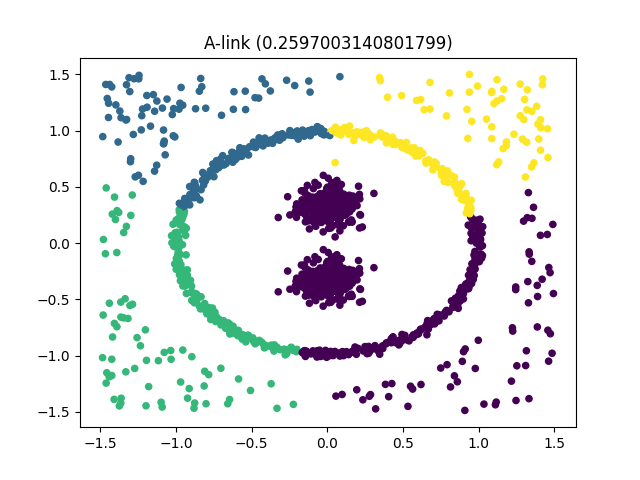
\includegraphics[width=\textwidth]{../results/plots/dataset_0/A-link_clustering.png}
    \end{subfigure}
    \hfill
    \begin{subfigure}[b]{0.32\textwidth}
        \centering
        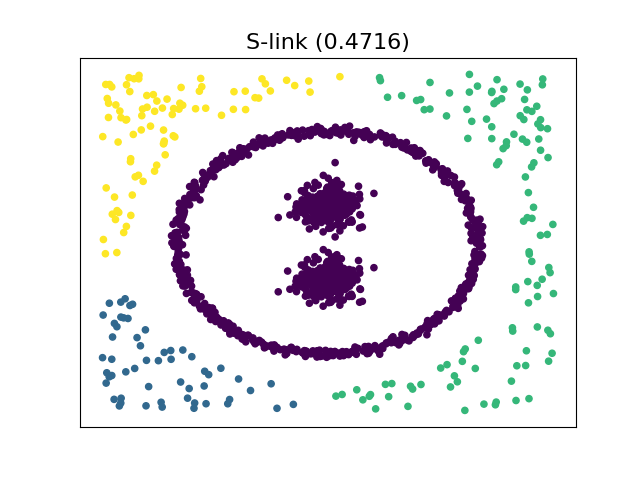
\includegraphics[width=\textwidth]{../results/plots/dataset_0/S-link_clustering.png}
    \end{subfigure}
    \hfill
    \begin{subfigure}[b]{0.32\textwidth}
        \centering
        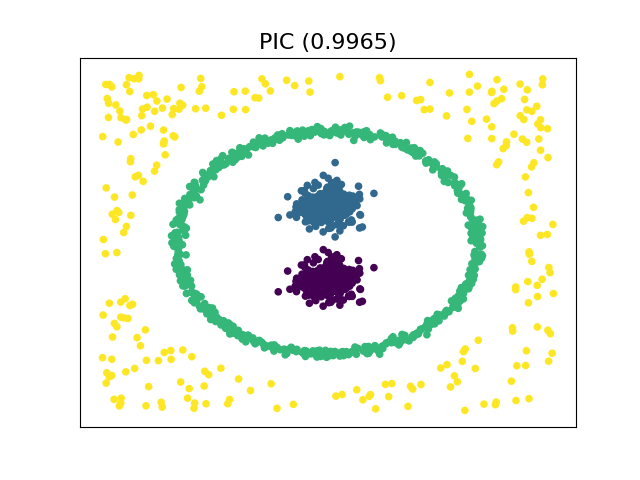
\includegraphics[width=\textwidth]{../results/plots/dataset_0/PIC_clustering.png}
    \end{subfigure}

    \begin{subfigure}[b]{0.32\textwidth}
        \centering
        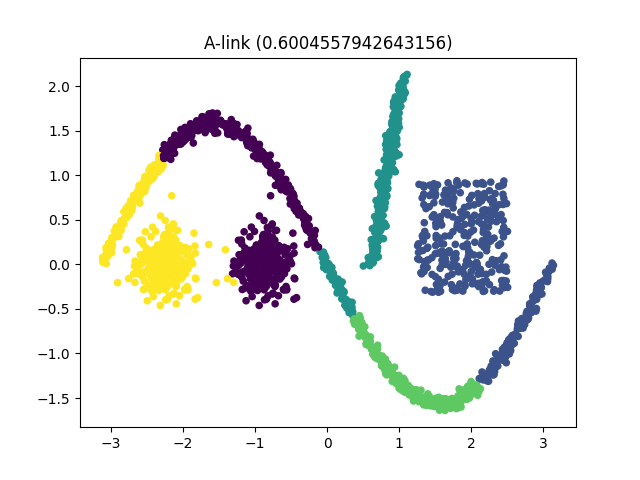
\includegraphics[width=\textwidth]{../results/plots/dataset_1/A-link_clustering.png}
    \end{subfigure}
    \hfill
    \begin{subfigure}[b]{0.32\textwidth}
        \centering
        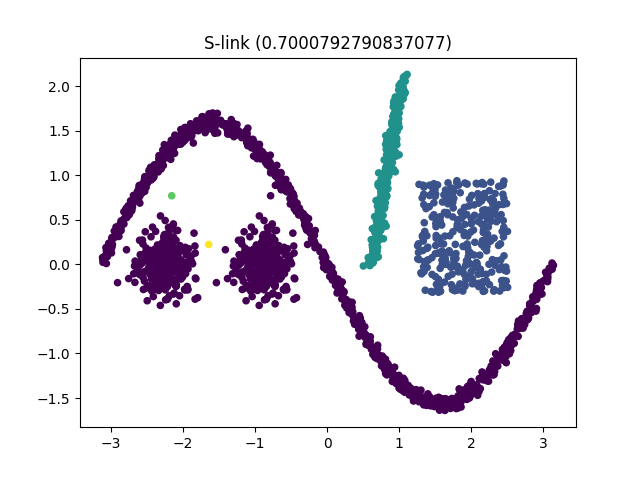
\includegraphics[width=\textwidth]{../results/plots/dataset_1/S-link_clustering.png}
    \end{subfigure}
    \hfill
    \begin{subfigure}[b]{0.32\textwidth}
        \centering
        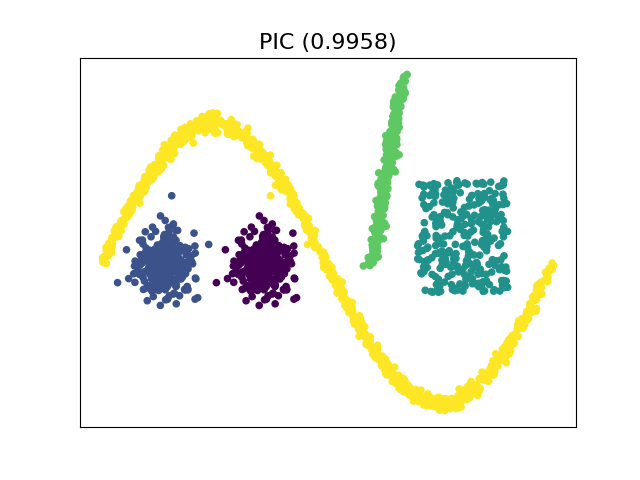
\includegraphics[width=\textwidth]{../results/plots/dataset_1/PIC_clustering.png}
    \end{subfigure}

    \begin{subfigure}[b]{0.32\textwidth}
        \centering
        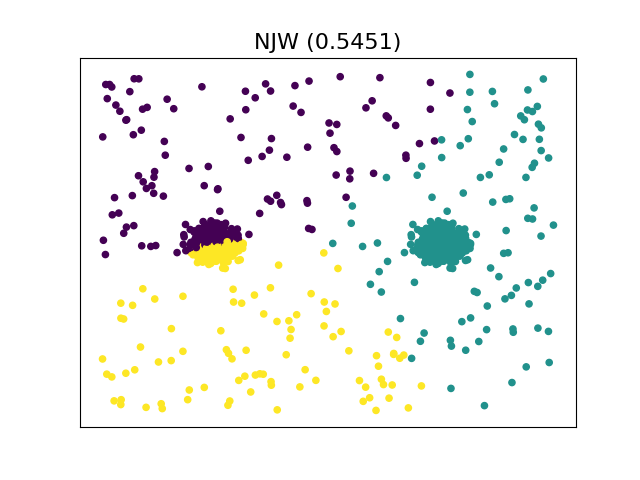
\includegraphics[width=\textwidth]{../results/plots/dataset_2/NJW_clustering.png}
    \end{subfigure}
    \hfill
    \begin{subfigure}[b]{0.32\textwidth}
        \centering
        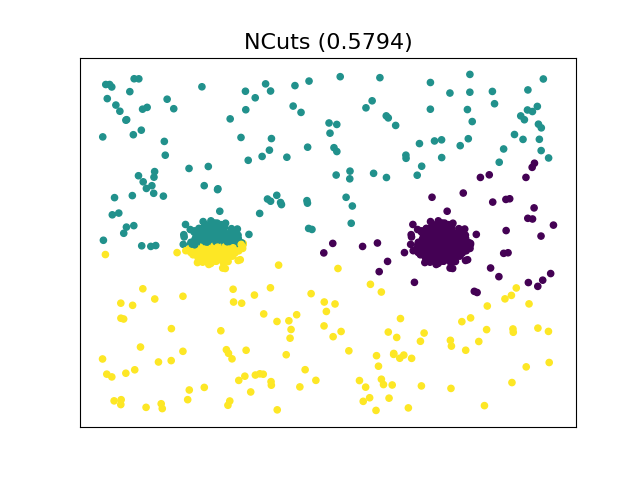
\includegraphics[width=\textwidth]{../results/plots/dataset_2/NCuts_clustering.png}
    \end{subfigure}
    \hfill
    \begin{subfigure}[b]{0.32\textwidth}
        \centering
        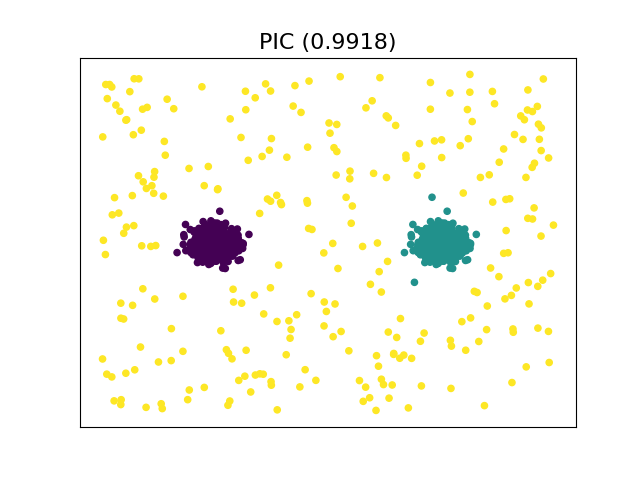
\includegraphics[width=\textwidth]{../results/plots/dataset_2/PIC_clustering.png}
    \end{subfigure}

    \caption{Clustering results on the three Synthetic Datasets (NMI scores in parentheses).}
    \label{fig:synthetic}
\end{figure*}

The results demonstrate PIC's ability to handle complex data structures. Particularly noteworthy is PIC's performance on Dataset 1, where it successfully identified both the dense clusters and the circular pattern despite the presence of noise. For Dataset 2, PIC effectively captured the sinusoidal and non-convex patterns, outperforming traditional algorithms that typically prefer convex clusters. Dataset 3 showcases PIC's robustness to noise, accurately separating the two main clusters from the surrounding noise.

\subsection{Imagery Datasets}
We evaluated PIC and 11 other clustering algorithms on three widely used image datasets:

\begin{enumerate}
    \item \textbf{MNIST}: Handwritten digits (0-4), with 5,139 samples and 784 dimensions (28$\times$28 pixels).
    \item \textbf{USPS}: Handwritten digits (0-9), with 9,298 samples and 256 dimensions (16$\times$16 pixels).
    \item \textbf{Caltech-256}: Reduced to six classes (hibiscus, ketch-101, leopards-101, motorbikes-101, airplanes-101, and faces-easy-101), with 600 samples and 4,200 dimensions (60$\times$70 grayscale images).
\end{enumerate}

\begin{table}[h]
\centering
\begin{tabular}{|l|c|c|c|}
\hline
\textit{NMI} & \textbf{MNIST} & \textbf{USPS} & \textbf{Caltech-256} \\
\hline
\textbf{PIC}       & \textbf{0.940} & 0.835 & \textbf{0.653} \\ \hline
\textbf{k-med}     & 0.318 & 0.553 & 0.315 \\ \hline
\textbf{A-link}    & 0.408 & 0.139 & 0.313 \\ \hline
\textbf{S-link}    & 0.002 & 0.002 & 0.019 \\ \hline
\textbf{C-link}    & 0.539 & 0.374 & 0.395 \\ \hline
\textbf{AP}        & 0.426 & 0.525 & 0.492 \\ \hline
\textbf{NCuts}     & 0.807 & 0.772 & 0.589 \\ \hline
\textbf{NJW}       & 0.898 & 0.784 & 0.529 \\ \hline
\textbf{CT}        & 0.634 & 0.439 & 0.181 \\ \hline
\textbf{Zell}      & 0.913 & \textbf{0.846} & 0.343 \\ \hline
\textbf{C-kernel}  & 0.780 & 0.768 & 0.521 \\ \hline
\textbf{D-kernel}  & 0.903 & \textbf{0.846} & 0.508 \\
\hline
\end{tabular}
\caption{Normalized Mutual Information (NMI) scores for all algorithms on image datasets. Higher values indicate better performance. Bold indicates best performance.}
\label{table:nmi}
\end{table}

\begin{table}[h]
\centering
\begin{tabular}{|l|c|c|c|}
\hline
\textit{CE} & \textbf{MNIST} & \textbf{USPS} & \textbf{Caltech-256} \\
\hline
\textbf{PIC}       & \textbf{0.016} & 0.269 & 0.307 \\ \hline
\textbf{k-med}     & 0.534 & 0.373 & 0.607 \\ \hline
\textbf{A-link}    & 0.573 & 0.778 & 0.665 \\ \hline
\textbf{S-link}    & 0.779 & 0.833 & 0.828 \\ \hline
\textbf{C-link}    & 0.280 & 0.601 & 0.507 \\ \hline
\textbf{AP}        & 0.960 & 0.934 & 0.705 \\ \hline
\textbf{NCuts}     & 0.115 & 0.356 & 0.328 \\ \hline
\textbf{NJW}       & 0.033 & 0.269 & \textbf{0.290} \\ \hline
\textbf{CT}        & 0.493 & 0.615 & 0.747 \\ \hline
\textbf{Zell}      & 0.027 & 0.197 & 0.680 \\ \hline
\textbf{C-kernel}  & 0.129 & 0.269 & 0.368 \\ \hline
\textbf{D-kernel}  & 0.029 & \textbf{0.132} & 0.315 \\
\hline
\end{tabular}
\caption{Clustering Error (CE) scores for all algorithms on image datasets. Lower values indicate better performance. Bold indicates best performance.}
\label{table:ce}
\end{table}

Looking at the results in Tables \ref{table:nmi} and \ref{table:ce}, we observe that:

\begin{itemize}
    \item \textbf{MNIST}: PIC achieved the highest NMI (0.940) and lowest CE (0.016), significantly outperforming other methods. This suggests that PIC effectively captures the intrinsic manifold structure of the handwritten digits.
    
    \item \textbf{USPS}: PIC performed well with an NMI of 0.835, though slightly behind the Diffusion kernel (D-kernel) and Zell methods which both achieved an NMI of 0.846. In terms of CE, D-kernel had the best performance (0.132), followed by Zell (0.197) and PIC (0.269). These results still show strong performance for PIC.
    
    \item \textbf{Caltech-256}: PIC significantly outperformed all other methods with an NMI of 0.653. For CE, NJW had the lowest value (0.290), followed closely by PIC (0.307). This demonstrates PIC's ability to handle higher-dimensional image data with complex visual patterns.
\end{itemize}

Our results largely align with those reported in the original paper, with PIC consistently performing as one of the top methods across datasets. However, we observed some differences:

\begin{enumerate}
    \item On the USPS dataset, our implementation shows D-kernel and Zell slightly outperforming PIC, whereas the original paper reported PIC as the best method. This discrepancy might be due to differences in the dataset composition (9,298 samples in our case versus 11,000 mentioned in the paper), or in each of our custom implementations (since these algorithms are not supported by stardard libraries).
    
    \item For Caltech-256, we achieved similar relative performance between methods, though our absolute scores differ from the paper, likely due to different preprocessing approaches.
\end{enumerate}

\subsection{Issues Encountered}
Several challenges were encountered during the attempt to reproduce the original paper's experiments with the highest fidelity possible:

\begin{enumerate}
    \item \textbf{Synthetic Dataset Generation}: The original paper did not provide clear guidelines for synthetic dataset generation. Considerable tuning was required to create datasets in which the PIC algorithm exhibited the behaviors described in the paper.
    
    \item \textbf{Algorithm Implementation}: Implementing all 11 comparison algorithms was challenging, requiring adaptation of existing libraries and development of custom implementations, since not all of them are supported by stardard Python libraries.
    
    \item \textbf{Dataset Availability}: Two datasets mentioned in the original paper were not available: FRGC-T requires restricted access, and PubFig is no longer publicly available.
    
    \item \textbf{Dataset Discrepancies}: The USPS dataset contained 9,298 samples instead of the 11,000 mentioned in the paper.
    
    \item \textbf{Preprocessing Ambiguity}: For Caltech-256, the paper stated a dimensionality of 4,200 but did not specify how images of different sizes were processed. We adopted a 60$\times$70 grayscale representation.
\end{enumerate}

Despite these challenges, our implementation successfully reproduced the main findings of the original paper, confirming PIC's effectiveness for clustering tasks, especially on datasets with complex manifold structures.

\subsection{Additional Experiments}
To further evaluate PIC's performance beyond the original paper's scope, we conducted additional experiments focusing on different evaluation criteria and datasets, and an analysis on the algorithm's scalability. These experiments aim to provide a more comprehensive understanding of PIC's strengths and limitations across varied clustering scenarios.

\subsubsection{Additional Evaluation Criteria}
In the original experiments, only external evaluation criteria are used (NMI and CE). We propose to include an internal evaluation metric to provide a more comprehensive assessment of clustering quality. We chose the Silhouette score due to its ability to measure both cluster cohesion and separation, as well as being well-suited for visualization purposes.

We evaluated the Silhouette scores of all algorithms on the image datasets, and the results are shown in Table \ref{table:silhouette}.

\begin{table}[h]
    \centering
    \begin{tabular}{|l|c|c|c|}
    \hline
    \textit{Silhouette} & \textbf{MNIST} & \textbf{USPS} & \textbf{Caltech-256} \\
    \hline
    \textbf{PIC}       & 0.106 & 0.024 & 0.129 \\ \hline
    \textbf{k-med}     & 0.101 & 0.087 & 0.139 \\ \hline
    \textbf{A-link}    & 0.103 & 0.095 & \textbf{0.174} \\ \hline
    \textbf{S-link}    & -0.010 & 0.047 & 0.035 \\ \hline
    \textbf{C-link}    & 0.093 & 0.040 & 0.101 \\ \hline
    \textbf{AP}        & 0.060 & 0.078 & 0.063 \\ \hline
    \textbf{NCuts}     & 0.084 & 0.086 & 0.149 \\ \hline
    \textbf{NJW}       & \textbf{0.111} & 0.116 & 0.114 \\ \hline
    \textbf{CT}        & 0.009 & -0.212 & -0.159 \\ \hline
    \textbf{Zell}      & 0.109 & 0.114 & 0.057 \\ \hline
    \textbf{C-kernel}  & 0.078 & 0.080 & 0.122 \\ \hline
    \textbf{D-kernel}  & 0.107 & \textbf{0.147} & 0.112 \\
    \hline
    \end{tabular}
    \caption{Silhouette scores for all algorithms on image datasets. Higher values indicate better performance. Bold indicates best performance.}
    \label{table:silhouette}
\end{table}

High Silhouette scores indicate cohesive (convex) and well-separated clusters. Therefore, the Silhouette scores reveal an interesting pattern: while PIC achieves outstanding NMI values, it doesn't consistently produce the highest Silhouette scores. This discrepancy actually highlights PIC's strength in identifying non-convex and complex cluster structures that better represent the true data distribution, even though such clusters may not appear as well-separated by internal convexity-based evaluation criteria like Silhouette.

\subsubsection{Additional Datasets}
The original paper only tests the PIC algorithm on synthetic data and on imagery datasets, we included as well the Iris and the Wisconsin Breast Cancer datasets. These widely-used benchmark datasets allow us to evaluate PIC's performance on lower-dimensional, well-structured data compared to the high-dimensional image datasets. The results are shown in Tables \ref{table:nmi_additional}, \ref{table:ce_additional}, and \ref{table:silhouette_additional}.

\begin{table}[h]
    \centering
    \begin{tabular}{|l|c|c|}
        \hline
        \textit{NMI} & \textbf{Iris} & \textbf{Breast Cancer} \\
        \hline
        \textbf{PIC}       & \textbf{0.806} & 0.409 \\ \hline
        \textbf{k-med}     & 0.758 & \textbf{0.498} \\ \hline
        \textbf{A-link}    & \textbf{0.806} & 0.088 \\ \hline
        \textbf{S-link}    & 0.717 & 0.005 \\ \hline
        \textbf{C-link}    & 0.722 & 0.088 \\ \hline
        \textbf{AP}        & 0.669 & 0.272 \\ \hline
        \textbf{NCuts}     & 0.786 & 0.420 \\ \hline
        \textbf{NJW}       & -- & 0.046 \\ \hline
        \textbf{CT}        & 0.397 & 0.414 \\ \hline
        \textbf{Zell}      & 0.786 & 0.414 \\ \hline
        \textbf{C-kernel}  & 0.777 & 0.299 \\ \hline
        \textbf{D-kernel}  & 0.763 & 0.420 \\
        \hline
        \end{tabular}
    \caption{NMI scores on additional datasets.}
    \label{table:nmi_additional}
\end{table}

\begin{table}[h]
    \centering
    \begin{tabular}{|l|c|c|}
        \hline
        \textit{CE} & \textbf{Iris} & \textbf{Breast Cancer} \\
        \hline
        \textbf{PIC}       & \textbf{0.093} & 0.181 \\ \hline
        \textbf{k-med}     & 0.107 & \textbf{0.132} \\ \hline
        \textbf{A-link}    & \textbf{0.093} & 0.337 \\ \hline
        \textbf{S-link}    & 0.320 & 0.371 \\ \hline
        \textbf{C-link}    & 0.160 & 0.337 \\ \hline
        \textbf{AP}        & 0.487 & 0.801 \\ \hline
        \textbf{NCuts}     & \textbf{0.093} & 0.174 \\ \hline
        \textbf{NJW}       & -- & 0.374 \\ \hline
        \textbf{CT}        & 0.433 & 0.178 \\ \hline
        \textbf{Zell}      & \textbf{0.093} & 0.178 \\ \hline
        \textbf{C-kernel}  & 0.120 & 0.265 \\ \hline
        \textbf{D-kernel}  & 0.113 & 0.174 \\
        \hline
        \end{tabular}
    \caption{CE scores on additional datasets.}
    \label{table:ce_additional}
\end{table}

\begin{table}[h]
    \centering
    \begin{tabular}{|l|c|c|}
        \hline
        \textit{Silhouette} & \textbf{Iris} & \textbf{Breast Cancer} \\
        \hline
        \textbf{PIC}       & \textbf{0.554} & 0.401 \\ \hline
        \textbf{k-med}     & 0.553 & 0.692 \\ \hline
        \textbf{A-link}    & \textbf{0.554} & 0.691 \\ \hline
        \textbf{S-link}    & 0.512 & \textbf{0.799} \\ \hline
        \textbf{C-link}    & 0.514 & 0.691 \\ \hline
        \textbf{AP}        & 0.347 & 0.391 \\ \hline
        \textbf{NCuts}     & 0.552 & 0.408 \\ \hline
        \textbf{NJW}       & -- & 0.247 \\ \hline
        \textbf{CT}        & -0.052 & 0.405 \\ \hline
        \textbf{Zell}      & 0.551 & 0.405 \\ \hline
        \textbf{C-kernel}  & 0.550 & 0.304 \\ \hline
        \textbf{D-kernel}  & 0.553 & 0.408 \\
        \hline
        \end{tabular}
    \caption{Silhouette scores on additional datasets.}
    \label{table:silhouette_additional}
\end{table}

Comment results.

Introduce Silhouette plots of PIC and reference Figure \ref{fig:silhouette}.

\begin{figure*}[htb]
    \centering
    \begin{subfigure}[b]{0.49\textwidth}
        \centering
        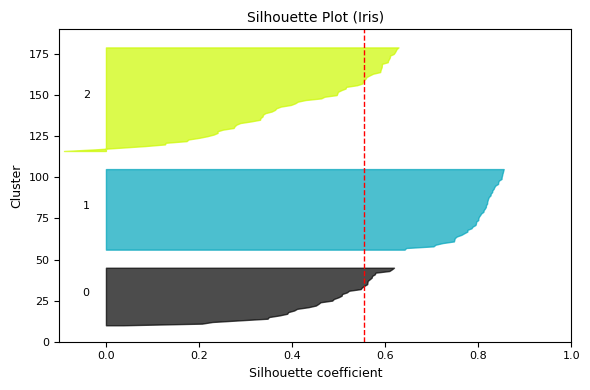
\includegraphics[width=\textwidth]{../results/plots/Iris.png}
    \end{subfigure}
    \hfill
    \begin{subfigure}[b]{0.49\textwidth}
        \centering
        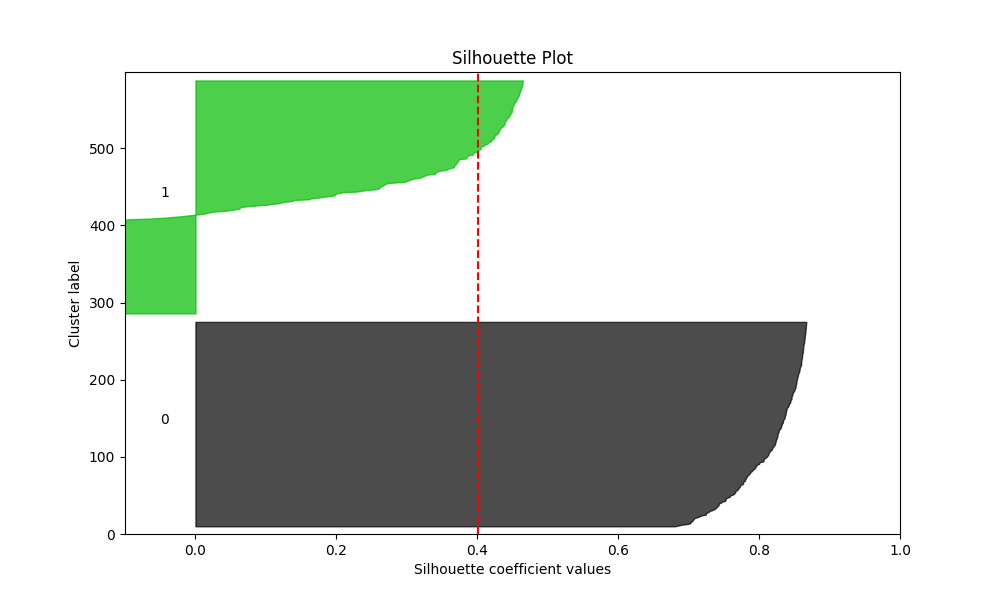
\includegraphics[width=\textwidth]{../results/plots/Breast-Cancer.png}
    \end{subfigure}

    \caption{Silhouette plots of PIC for the Iris and Breast Cancer datasets.}
    \label{fig:silhouette}
\end{figure*}

\subsubsection{Scalability Analysis}

\begin{table*}[h]
    \centering
    \begin{tabular}{|l|c|c|c|c|c|}
    \hline
     & \textbf{MNIST} & \textbf{USPS} & \textbf{Caltech-256} & \textbf{Iris} & \textbf{Breast Cancer} \\
    \hline
    \textbf{\# of samples} & 5,139 & 9,298 & 600 & 150 & 569 \\ \hline
    \textbf{\# of clusters} & 5 & 10 & 6 & 3 & 2 \\ \hline
    \textbf{Dimensionality} & 784 & 256 & 4,200 & 4 & 30 \\ \hline
    \textbf{PIC Runtime (s)} & 256.1 & 854.7 & 1.5 & 0.3 & 4.2 \\ \hline
    \end{tabular}
    \caption{Runtime of PIC on different datasets with varying sizes and dimensionalities.}
    \label{table:time}
\end{table*}

The original paper states that the PIC algorithm scales linearly with the number of clusters. However, it does not mention the algorithm's scalability with respect to the number of samples or dimensions. To investifate this, we recorded the runtime of PIC on each of the tested datasets, which have different number of samples, clusters and dimensions. The results are shown in Table \ref{table:time}.

The results show that PIC's runtime does not seem to be affected by the dimensionality of the dataset in any significant way, since the Caltech-256 dataset has the highest number of dimensions and yet has the lowest runtime by a wide margin. However, the runtime does greatly increase with the number of samples, as seen in the MNIST and USPS datasets. The number of clusters could also have an impact, but it does not seem to be as significant as that of the number of samples.


\section{Conclusion}
Your conclusion here.

\bibliographystyle{unsrt}
\bibliography{references}

\end{document}